\documentclass{article}
\usepackage{graphicx}
\usepackage[margin=1.5cm]{geometry}
\usepackage{amsmath}

\begin{document}
\twocolumn

\title{Friday warm-up: Kinematics III, and the Cross-Product}
\author{Prof. Jordan C. Hanson}

\maketitle

\begin{figure}
\centering
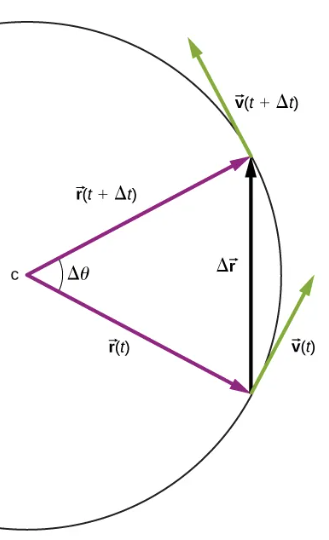
\includegraphics[width=0.15\textwidth]{figures/circle1.png}
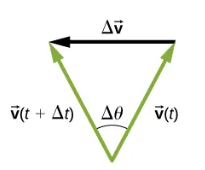
\includegraphics[width=0.15\textwidth]{figures/circle2.png}
\caption{\label{fig:1} Geometric picture of centripetal acceleration.}
\end{figure}

\begin{figure}
\centering
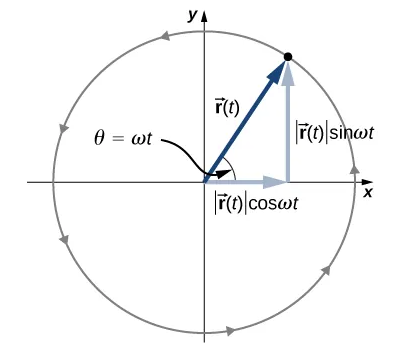
\includegraphics[width=0.25\textwidth]{figures/circular.png}
\caption{\label{fig:2} Algebraic picture of centripetal acceleration.}
\end{figure}

\section{Memory Bank}

\begin{enumerate}
\item $s = r\theta$ ... Arc length $s$, radius $r$, and the radian, $\theta$.
\item $\vec{r}(t) = r \cos(\omega t) \hat{i} + r \sin(\omega t) \hat{j}$
\item $\omega = \Delta \theta / \Delta t$ ... Average \textit{angular} velocity
\item $\vec{v} = \vec{\omega} \times \vec{r}$ ... Relationship between \textit{tangential} velocity, radius, and \textit{angular} velocity
\item The \textbf{cross-product}:
\begin{itemize}
\item $\hat{i} \times \hat{j} = \hat{k}$
\item $\hat{k} \times \hat{i} = \hat{j}$
\item $\hat{j} \times \hat{k} = \hat{i}$
\item Non-alphabetical order: multiply by -1. For example, $\hat{k} \times \hat{i} = -\hat{j}$
\item $\hat{i} \times \hat{i} = 0$, $\hat{j} \times \hat{j} = 0$, $\hat{k} \times \hat{k} = 0$
\end{itemize}
\end{enumerate}

\section{The Cross Product of Vectors}

\begin{enumerate}
\item Multiply these vectors using the \textit{cross-product}: (a) $\vec{v}_1 = 2 \hat{i}$, and $\vec{v}_2 = 3\hat{j}$. (b) $\vec{v}_1 = 2 \hat{i} + 2 \hat{j}$, and $\vec{v}_2 = \hat{i} - \hat{j}$. \\ \vspace{0.5cm}
\end{enumerate}

\section{Kinematics III}

\begin{enumerate}
\item In Fig. \ref{fig:1}, the angle $\Delta \theta$ is the same in both triangles. (a) Why does $\Delta v/v = \Delta r/r$? (b) Multiply both sides by $v$, to obtain $\Delta v = v/r\Delta r$.  Now divide both sides by $\Delta t$, and take the limit that $\Delta t \to 0$.  What is the result? (c) Let $s(t) = r\theta (t)$.  Take the derivative of both sides, and let $d\theta(t)/dt = \omega$.  What do you find? (d) Now eliminate $v$ in favor of $\omega$ in the expression you derived for the acceleration.  (d) Suppose a warrior is using a \textit{sling} to hurl a stone at an enemy.  The stone circles above his head with radius $r=1$ m.  If the stone makes 1 revolution every 0.25 seconds, what is its speed and acceleration? \\ \vspace{3.5cm}
\item Consider Fig. \ref{fig:1}.  The angle $\theta(t) = \omega t$ describes the position of a system circling the origin at constant speed.  Prove the following
\begin{align}
\vec{r}(t) &= r \cos(\omega t) \hat{i} + r \sin(\omega t) \hat{j} \\
\vec{a} &= -\omega^2 \vec{r}
\end{align} \vspace{1cm}
\item (a) Draw a diagram of a circle in the xy-plane, centered at the origin, and draw the \textit{axis of rotation} along the z-axis. (b) Show that if $\vec{v}$ is tangent to the circle, and $\vec{r}$ is the displacement from the origin, $\vec{\omega}$ constantly points in the z-direction, if $\vec{v} = \vec{\omega} \times \vec{r}$.
\end{enumerate}

\end{document}
